\section{Concepts and terminology}

Almost all of the information in this chapter is taken from the official Chef wiki\cite{chef_wiki}.

\subsection{Chef-client}

A chef-client is an agent that runs locally on every node that is registered with the server. When a chef-client is run, it will perform all of the steps that are required to bring the node into the expected state, including:

\begin{itemize}
  \item Registering and authenticating the node with the server
  \item Building the node object
  \item Synchronizing cookbooks
  \item Compiling the resource collection by loading each of the required cookbooks, including recipes, attributes, and all other dependencies
  \item Taking the appropriate and required actions to configure the node
  \item Looking for exceptions and notifications, handling each as required
\end{itemize}

\subsection{Nodes}

A node is any physical, virtual, or cloud machine that is configured to be maintained by a chef-client.

\subsection{Chef Solo}

Chef Solo is simple way to begin working with Chef. It is an open source version of the chef-client that allows using cookbooks with nodes without requiring access to a server. Chef Solo runs locally and requires that a cookbook (and any of its dependencies) be on the same physical disk as the node. It is a limited-functionality version of the chef-client and does not support the following:

\begin{itemize}
  \item Node data storage
  \item Search indexes
  \item Centralized distribution of cookbooks
  \item A centralized API that interacts with and integrates infrastructure components
  \item Authentication or authorization
  \item Persistent attributes
\end{itemize}

\subsection{Chef Server}

The server acts as a hub for configuration data. The server stores cookbooks, the policies that are applied to nodes, and metadata that describes each registered node that is being managed by the chef-client. Nodes use the chef-client to ask the server for configuration details, such as recipes, templates, and file distributions. The chef-client then does as much of the configuration work as possible on the nodes themselves (and not on the server). This scalable approach distributes the configuration effort throughout the organization.

The diagram~\ref{fig:overview_chef_draft} shows the relationships between the various elements of Chef, including the nodes, the server, and the workstations. These elements work together to provide the chef-client the information and instruction that it needs so that it can do its job.

\begin{figure}[ht!]
  \center{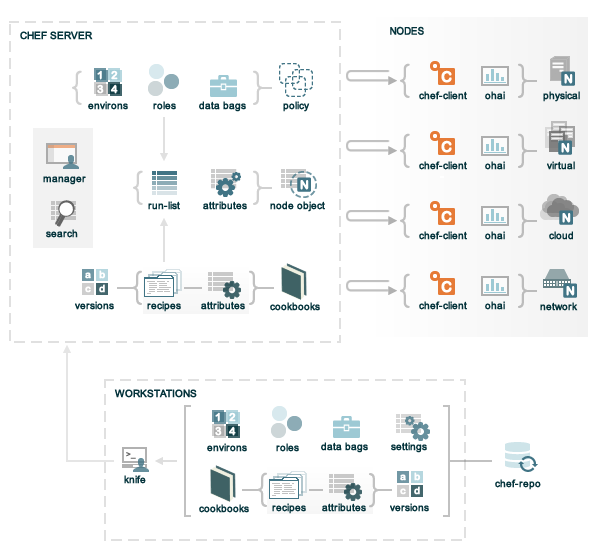
\includegraphics[width=1\textwidth]{overview_chef_draft}}
  \caption{Chef Infrastructure}
  \label{fig:overview_chef_draft}
\end{figure}

\subsection{Chef-repo}

The chef-repo is the location in which the following data objects are stored:

\begin{itemize}
  \item Cookbooks (including recipes, versions, cookbook attributes, resources, providers, libraries, and templates)
  \item Roles
  \item Data bags
  \item Environments
  \item Configuration files (for clients, workstations, and servers)
\end{itemize}

The chef-repo is located on a workstation and should be synchronized with a version control system, such as git. All of the data in the chef-repo should be treated like source code.

\subsection{Knife}

Knife is a command-line tool that provides an interface between a local chef-repo and the server. Knife helps users to manage:

\begin{itemize}
  \item Nodes
  \item Cookbooks and recipes
  \item Roles
  \item Stores of JSON data (data bags), including encrypted data
  \item Environments
  \item Cloud resources, including provisioning
  \item The installation of the chef-client on management workstations
  \item Searching of indexed data on the server
\end{itemize}

\subsection{Workstations}

A workstation is a computer that is configured to run Knife, to synchronize with the chef-repo, and interact with a single server. The workstation is the location from which most users will do most of their work, including:

\begin{itemize}
  \item Developing cookbooks and recipes (and authoring them using Ruby)
  \item Keeping the chef-repo synchronized with version source control
  \item Using Knife to upload items from the chef-repo to the server
  \item Configuring organizational policy, including defining roles and environments and ensuring that critical data is stored in data bags
  \item Interacting with nodes, as (or when) required, such as performing a bootstrap operation
\end{itemize}

\subsection{Environments}

An environment is a way to map an organization's real-life workflow to what can be configured and managed when using server. Every organization begins with a single environment called the \_default environment, which cannot be modified (or deleted). Additional environments can be created to reflect each organization’s patterns and workflow. For example, creating production, staging, testing, and development environments. Generally, an environment is also associated with one (or more) cookbook versions.

\subsection{Role}

A role is a way to define certain patterns and processes that exist across nodes in an organization as belonging to a single job function. Each role consists of zero (or more) attributes and a run list. Each node can have zero (or more) roles assigned to it. When a role is run against a node, the configuration details of that node are compared against the attributes of the role, and then the contents of that role’s run list are applied to the node’s configuration details. When a chef-client runs, it merges its own attributes and run lists with those contained within each assigned role.

\subsection{Cookbooks}

A cookbook is the fundamental unit of configuration and policy distribution. Each cookbook defines a scenario, such as everything needed to install and configure MySQL, and then it contains all of the components that are required to support that scenario, including:

\begin{itemize}
  \item Attribute values that are set on nodes
  \item Definitions that allow the creation of reusable collections of resources
  \item File distributions
  \item Libraries that extend the chef-client and/or provide helpers to Ruby code
  \item Recipes that specify which resources to manage and the order in which those resources will be applied
  \item Custom resources and providers
  \item Templates
  \item Versions
  \item Metadata about recipes (including dependencies), version constraints, supported platforms, and so on
\end{itemize}

\subsection{Recipes}

A recipe is the most fundamental configuration element within the organization. A recipe:

\begin{itemize}
  \item Is authored using Ruby, which is a programming language designed to read and behave in a predictable manner
  \item Is mostly a collection of resources in a Ruby syntax with some helper code around it
  \item Must define everything that is required to configure part of a system
  \item Must be stored in a cookbook
  \item May be included in a recipe
  \item May use the results of a search query and read the contents of a data bag (including an encrypted data bag)
  \item May have a dependency on one (or more) recipes
  \item May be tagged to facilitate the creation of arbitrary groupings that exist outside of the normal naming conventions an organization may have
  \item Must be added to a run-list before it can be used by the chef-client
  \item Is always executed in the same order as listed in a run-list
\end{itemize}

\subsection{Attribute}

An attribute is a specific detail about a node. Attributes are used by the chef-client to understand:

\begin{itemize}
  \item The current state of the node
  \item What the state of the node was at the end of the previous chef-client run
  \item What the state of the node should be at the end of the current chef-client run
\end{itemize}

Attributes are defined by:

\begin{itemize}
  \item The state of the node itself
  \item Cookbooks (in attribute files and/or recipes)
  \item Roles
  \item Environments
\end{itemize}

\subsection{Template}

A cookbook template is a file written in a markup language that allows the contents of a file to be dynamically generated based on variables or complex logic. Templates can contain Ruby expressions and statements. Templates are a great way to manage configuration files across an organization. A template requires a template resource being added to a recipe and then a corresponding Embedded Ruby (ERB) template being added to a cookbook.

\subsection{Data Bags}

A data bag is a global variable that is stored as JSON data and is accessible from a server. A data bag is indexed for searching and can be loaded by a recipe or accessed during a search. The contents of a data bag can vary, but they often include sensitive information (such as database passwords).

\subsection{Run-lists}

A run-list is an ordered list of roles and/or recipes that are run in an exact order. A run-list is always specific to the node on which it runs, though it is possible for many nodes to have run-lists that are similar or even identical. The items within a run-list are maintained using Knife and are uploaded to the server and stored as part of the node object for each node. The chef-client always configures a node in the exact order specified by its run-list and will never run the same recipe twice.

\subsection{Policy}

Policy settings can be used to map business and operational requirements, such as process and workflow, to settings stored on the server:

\begin{itemize}
  \item Roles define server types, such as <<web server>> or <<database server>>
  \item Environments define process, such as <<dev>>, <<staging>>, or <<production>>
  \item Certain types of data—passwords, user account data, and other sensitive items—can be placed in data bags, which are located in a secure sub-area on the server that can only be accessed by nodes that authenticate to the server with the correct SSL certificates
  \item The cookbooks in which organization-specific configuration policies are maintained
\end{itemize}

\subsection{Ohai}

Ohai is a tool that is used to detect attributes on a node, and then provide these attributes to the chef-client at the start of every chef-client run. Ohai is required by the chef-client and must be present on a node. The types of attributes Ohai collects include:

\begin{itemize}
  \item Platform details
  \item Networking usage
  \item Memory usage
  \item Processor usage
  \item Kernel data
  \item Host names
  \item Fully qualified domain names
  \item Other configuration details
\end{itemize}

Attributes that are collected by Ohai are automatic attributes, in that these attributes are used by the chef-client to ensure that these attributes remain unchanged after the chef-client is done configuring the node.